

\title[Systems Engineering]{ System Science} 




\begin{frame}
\frametitle{Sub System Interconnect }


\begin{figure}
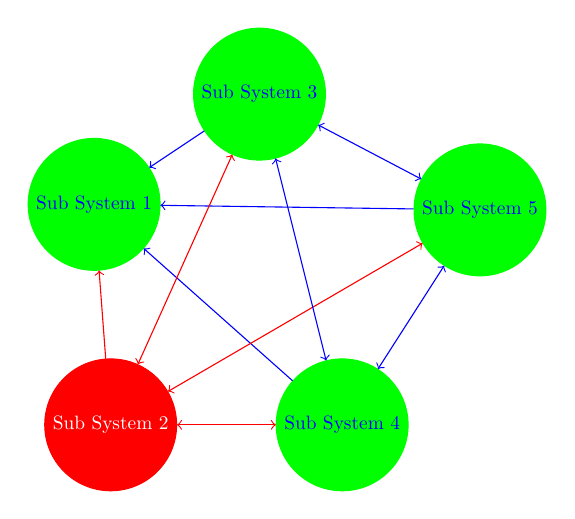
\begin{tikzpicture}[scale=0.7,transform shape,every state/.style={minimum width={1cm},thick,align=center},state/.style={circle, draw, minimum size=1cm}]
\node[state] [color=green, fill=green] (1) {{\color{blue}  Sub System 1}};
\node[state] [color=green, fill=green]  at (3, 2) (3) {
{\color{blue} Sub  System 3}   };
\node[state] [color=green, fill=green] at (7, -0.1) (5) {{\color{blue}  Sub System 5}};
\node[state] [color=red, fill=red] at (0.3,-4) (2) {{\color{white}  Sub System 2}};
\node[state] [color=green, fill=green] at (4.5,-4) (4) {{\color{blue}  Sub System 4}};
					
					\draw[<-] [draw = red](1) -- node [ midway,above] {} (2);
					\draw[<-] [draw = blue] (1) -- node [midway,below] {} (3);
					\draw[<-] [draw = blue] (1) -- node [midway,below] {} (4);
					\draw[<-] [draw = blue] (1) -- node [midway,below] {} (5);
					
					\draw[<->] [draw = red] (2) -- node [midway,below] {} (3);
					\draw[<->] [draw = red] (2) -- node [midway,below] {} (4);
					\draw[<->] [draw = red] (2) -- node [midway,below] {} (5);
					
					\draw[<->] [draw = blue] (3) -- node [midway,below] {} (4);
					\draw[<->] [draw = blue] (3) -- node [midway,below] {} (5);
					
					\draw[<->] [draw = blue] (4) -- node [midway,below] {} (5);
				\end{tikzpicture}
		
\caption{Red is faulty System, Green is good System}
\label{rgpic}
\end{figure}
\end{frame}


\newpage
\begin{frame}
\frametitle{ System Science }
\begin{block}{ Validating Requirements from a Persons}

 \vspace{2cm}

  \colorbox{cyan}{ \textcolor{white}{   BI  } }

\end{block}
\end{frame}



\newpage
\begin{frame}
\frametitle{ System Science }
\begin{block}{ Mission Critical and Cost is not Issue}

 \vspace{2cm}

  \colorbox{red}{ \textcolor{white}{  Redundant Resources  } }

\end{block}
\end{frame}


 \newpage
 
\begin{frame}
\frametitle{ System Science }

\begin{figure}
 \centering
 \tikz \node [scale=1.4, inner sep=0]  {
\begin{tikzpicture}
	[auto,
	cloudY/.style ={draw=blue!10, thick, circle,fill=yellow,
		minimum height=1em},
	cloudtummy/.style ={draw=white, circle,fill=white,
		minimum height= 0.1em},
	line/.style ={draw=blue!20, thick, -latex',shorten >=2pt},
	lineR/.style ={draw=red, thick, -latex',shorten >=2pt},
	cloudG/.style ={draw=blue!10, thick, circle,fill=green,
		minimum height=1em}]
	
        \matrix (magic) [matrix of nodes,ampersand replacement=\&, column sep=7mm,row sep=2mm]
	{
		
		% row 1
		
	\& 		\node [cloudG] (NN1g) {$  v_1 $}; \&   \&   \&   \\
		
		\&  \& \&	\node [cloudY] (NN1y) {$  h_{11} $};  \&  \node [cloudY] (NN12y) {$  h_{12} $};   \\
  
        		
		\& 		\node [cloudG] (NN2g) {$  v_2 $}; \&    \&  \&   \\
		
		\&  \& \&	\node [cloudY] (NN2y) {$  h_{21} $};  \&    \node [cloudY] (NN22y) {$  h_{22} $};    \\
		
		\& 		\node [cloudG] (NN3g) {$  v_3 $}; \&   \&  \&  \\
		
		\&  \& \&	\node [cloudY] (NN3y) {$  h_{31} $};  \&     \node [cloudY] (NN32y) {$  h_{32} $};   \\
		
		\& 		\node [cloudG] (NN4g) {$  v_4 $}; \&    \&  \&  \\
	}; 
	
	\begin{scope}[every path/.style=line ]
		
		
		\path [draw, <->] (NN1g) --  (NN1y);
		\path [draw, <->] (NN2g) --  (NN1y);
		\path [draw, <->] (NN3g) --  (NN1y);
		\path [draw, <->] (NN4g) --  (NN1y);
		
		\path [draw, <->] (NN1g) --  (NN2y);
		\path [draw, <->] (NN2g) --  (NN2y);
		\path [draw, <->] (NN3g) --  (NN2y);
		\path [draw, <->] (NN4g) --  (NN2y);
		
		\path [draw, <->] (NN1g) --  (NN3y);
		\path [draw, <->] (NN2g) --  (NN3y);
		\path [draw, <->] (NN3g) --  (NN3y);
		\path [draw, <->] (NN4g) --  (NN3y);


        \path [draw, <->] (NN1y) --  (NN12y);
		\path [draw, <->] (NN1y) --  (NN22y);
		\path [draw, <->] (NN1y) --  (NN32y);

        \path [draw, <-> ] (NN2y) --  (NN12y);
		\path [draw, <-> ] (NN2y) --  (NN22y);
		\path [draw, <->] (NN2y) --  (NN32y);

        \path [draw, <->] (NN3y) --  (NN12y);
		\path [draw, <->] (NN3y) --  (NN22y);
		\path [draw, <-> ] (NN3y) --  (NN32y);
  
	
		
	\end{scope}
	
\end{tikzpicture}
};
  \caption{Neural Network Model : All resources are used }
    \label{fNNmodel1}
\end{figure}

\end{frame}


\begin{frame}
\frametitle{ System Science }

\begin{figure}
 \centering
\tikz \node [scale=1.4, inner sep=0]  {
\begin{tikzpicture}
	[
        scale=.3,
	cloudY/.style ={draw=blue!10, thick, circle,fill=yellow, minimum height=1em},
	cloudtummy/.style ={draw=white, circle,fill=white, minimum height= 0.1em},
	line/.style ={draw=blue!20, thick, -latex',shorten >=2pt},
	lineR/.style ={draw=red, thick, -latex',shorten >=2pt},
	cloudG/.style ={draw=blue!10, thick, circle,fill=green, minimum height=1em}
        ]
	
        \matrix (magic) [matrix of nodes,ampersand replacement=\&, column sep=7mm,row sep=2mm]
	{
		
		% row 1
		
	\& 		\node [cloudG] (NN1g) {$  v_1 $}; \&   \&   \&   \\
		
		\&  \& \&	\node [cloudY] (NN1y) {$  h_{11} $};  \&  \node [cloudY] (NN12y) {$  h_{12} $};   \\
  
        		
		\& 		\node [cloudG] (NN2g) {$  v_2 $}; \&    \&  \&   \\
		
		\&  \& \&	\node [cloudY] (NN2y) {$  h_{21} $};  \&    \node [cloudY] (NN22y) {$  h_{22} $};    \\
		
		\& 		\node [cloudG] (NN3g) {$  v_3 $}; \&   \&  \&  \\
		
		\&  \& \&	\node [cloudY] (NN3y) {$  h_{31} $};  \&     \node [cloudY] (NN32y) {$  h_{32} $};   \\
		
		\& 		\node [cloudG] (NN4g) {$  v_4 $}; \&    \&  \&  \\
	}; 
	
	\begin{scope}[every path/.style=line ]
		
		
		\path [draw, <->] (NN1g) --  (NN1y);
		\path [draw, <->] (NN2g) --  (NN1y);
		\path [draw, <->] (NN3g) --  (NN1y);
		\path [draw, <->] (NN4g) --  (NN1y);
		
		\path [draw, <->] (NN1g) --  (NN2y);
		\path [draw, <->] (NN2g) --  (NN2y);
		\path [draw, <->] (NN3g) --  (NN2y);
		\path [draw, <->] (NN4g) --  (NN2y);
		
		\path [draw, <->] [draw = blue ] (NN1g) --  (NN3y);
		\path [draw, <->] (NN2g) --  (NN3y);
		\path [draw, <->] (NN3g) --  (NN3y);
		\path [draw, <->] (NN4g) --  (NN3y);


        \path [draw, <->] (NN1y) --  (NN12y);
		\path [draw, <->] (NN1y) --  (NN22y);
		\path [draw, <->] (NN1y) --  (NN32y);

        \path [draw, <-> ] (NN2y) --  (NN12y);
		\path [draw, <-> ] (NN2y) --  (NN22y);
		\path [draw, <->] (NN2y) --  (NN32y);

        \path [draw, <->] [draw = blue ] (NN3y) --  (NN12y);
		\path [draw, <->] (NN3y) --  (NN22y);
		\path [draw, <-> ] (NN3y) --  (NN32y);
  
	
		
	\end{scope}
	
\end{tikzpicture}
};
  \caption{Neural Network Model :  Time Optimization}
    \label{fNNmodela}
\end{figure}


\end{frame}





\newpage
\begin{frame}
\frametitle{ System Science }

\begin{figure}[ht]
 \centering
 \tikz \node [scale=0.7, inner sep=0]  {
\begin{tikzpicture}[->,>=stealth']
	% First node
	% Use previously defined 'state' as layout (see above)
	% use tabular for content to get columns/rows
	% parbox to limit width of the listing
	\node[state, color = jgold] (QUERY) 
	{\begin{tabular}{l}
			\textbf{Sensor Sample Buffer}\\
			\parbox{4cm}{
				\begin{tabular}{|l|}
					\hline
					sample 1  \\ \hline
					sample 2  \\ \hline
					sample 3  \\ \hline
					sample 4 \\ \hline
					\ldots   \\ \hline
					sample k  \\ \hline
				\end{tabular}
			}\\[4em]
			\textbf{ (0, t) sec}\\
			\parbox{4cm}{k Samples in a Sensor}
	\end{tabular}};
	
	% Next node: RAKE
	\node[state,       % layout (defined above)
	node distance=6cm,     % distance to QUERY
	text width=4cm,        % max text width
	color = jgold2,
	right of=QUERY,        % Position is to the right of QUERY
	yshift=+3cm] (RAKE)    % move 3cm in y
	{%                     % posistion relative to the center of the 'box'
		\begin{tabular}{l}     % content
			\parbox{4cm}{Processing Element (PE) in a Sensor $ j$}
		\end{tabular}
	};
	
	% STATE ACK
	\node[state,
	below of=RAKE,
	node distance=2cm,
	color = blue,
	text width=3cm] (ACK) 
	{%
		\begin{tabular}{l}
			\textbf{ Measured Value}\\
			\parbox{2.8cm}{ Accuracy Range}
		\end{tabular}
	};
	
	% STATE EPC
	\node[state,
	above of=RAKE,
	color = brilliantrose,
	node distance=3cm] (EPC) 
	{%
		\begin{tabular}{l}
			Measured Value from other Sensors \\
			\parbox{4cm}{ (N-1 sensors) }
		\end{tabular}
	};
	
	% draw the paths and and print some Text below/above the graph
	\path (QUERY) edge[bend left=30]  node[anchor=south,above, color = DarkGreen2,
	text width=4cm]
	{
		\begin{tabular} {l}
			Store and  \\
			Share with PE
		\end{tabular}
	} (RAKE)
	(RAKE) edge                    (ACK)
	(EPC)  edge                    node[anchor=east,left,color = DarkGreen2,text width=3cm,xshift=1em]
	{
		\begin{tabular} {l}
			Processed Value  \\
			from other 
			sensors
		\end{tabular}
	} (RAKE)
	;
\end{tikzpicture}
};
    \caption{Brooks-Iyengar Algorithm}
    \label{traningBINmodel}
\end{figure}
\end{frame}
\newpage
\begin{frame}
\frametitle{ System Science }
\begin{block}{Diagram to Neural Network}

\url{https://towardsdatascience.com/backpropagation-step-by-step-derivation-99ac8fbdcc28}

\end{block}
\end{frame}



